\documentclass[10pt,a5paper]{book}
\usepackage[utf8]{inputenc}
\usepackage[english]{babel}
\usepackage{amsmath}
\usepackage{amsfonts}
\usepackage{amssymb}
\usepackage{geometry}
\usepackage{graphicx}
\usepackage{fancyhdr}
\usepackage{lipsum}
\usepackage{multirow}
\usepackage{verbatim}
\usepackage{xstring}
\usepackage{xcolor}

\pagestyle{fancy}

\definecolor{blue}{HTML}{115599}

\pagestyle{fancy}
\lhead{}
\rhead{Abstracts of ICCA10, August 4–9, 2014, Tartu, Estonia}

\newcommand{\abstract}[4]{
  \StrLeft{#1}{1}[\firstletter]
  \newpage
  \subsection*{\MakeUppercase{#3}}
  \subsubsection*{\scshape{#1 #2}}
  \addcontentsline{toc}{section}{
    \textit{\textbf{\firstletter. #2}}, #3
  }
  #4
}


\begin{document}

\begin{titlepage}

   \begin{center}
      \textcolor{blue}{ \Huge{ICCA10} }
      \textcolor{blue}{ \rule[1mm]{10.1cm}{0.7pt} } 
      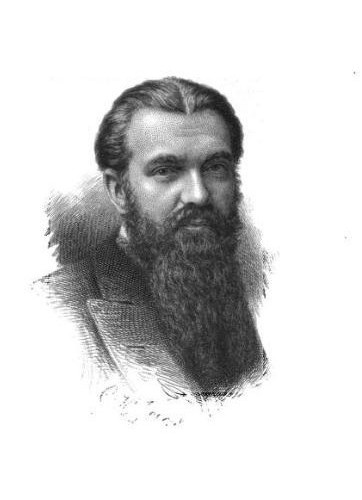
\includegraphics[scale=2]{clifford_large.jpg}\\      
      \textcolor{blue}{ \huge{\textbf{Book of Abstracts}} } \\
      \vspace{1cm}
      \textcolor{blue}{ \Large{$10^{\text{th}}$ International Conference on Clifford Algebras and their Applications in Mathematical Physics} } \\
      \vspace{1.4cm}
      \textcolor{blue}{ \small{\textbf{Tartu, Estonia \\ August 4–9, 2014}} }\\
   \end{center}
\end{titlepage}

\tableofcontents

\title{Abstracts of ICCA10, Tartu, 4–9 August 2014}

\newpage

ABSTRACTS-LOCATION

\end{document}